
\section{Performance Advisories}
\label{mbox2:sec:advisories}

The previous section has shown that, when used globally, miniboxed generics provide two key invariants that ensure primitive values are always passed using the miniboxed (long integer) encoding:

\begin{itemize}
\item Instantiations of miniboxed classes use the most specific variant (e.g. a value of type |Node[Int]| has runtime class |Node_M|);
\item Methods called on a miniboxed class use the most specific specialization available (e.g. a runtime class |Node_M| always receives calls to the miniboxed |head_M| accessor)
\end{itemize}

The presence of erasure and wildcard-type abstractions (such as |Node[_]|) leads to violations of these two invariants: the reference variant of a miniboxed class may be instantiated in place of a miniboxed variant or the method called may not be the most specific one available. In both cases, the compilation scheme is resilient, producing correct results, at the expense of performance regressions, caused by boxing primitive types.

There key to avoiding these subtle performance regressions is to intercept the class instantiations and method calls that violate the invariant and report actionable advisories to the users, in the form of compiler warnings. Luckily, all the information necessary to detect invariant violations is available during compilation.



\subsection{Performance Advisories Overview}



Advisories are most commonly triggered by interacting with erased or specialized generics, but can also be caused by technical or design limitations. There are as many as ten different performance advisories implemented in the miniboxing plugin, but in order to focus on the concept, we will only look at the three most common advisories, two of which are caused by the interaction with erased generics. To show exactly how the slowdowns occur, we can take the following piece of code:

\begin{lstlisting-nobreak}
 def foo[`@miniboxed` T](t: T): T = bar(t)
 def bar[`@miniboxed` U](u: U): U = baz(u)
 def baz[`@miniboxed` V](v: V): V = v
\end{lstlisting-nobreak}

The code is compiled to:

\begin{lstlisting-nobreak}
 def foo(t: Object): Object = bar(t)
 def bar(u: Object): Object = baz(u)
 def baz(v: Object): Object = v
 def foo`_M`(..., t: long): long = bar`_M`(..., t)
 def bar`_M`(..., u: long): long = baz`_M`(..., u)
 def baz`_M`(..., v: long): long = v
\end{lstlisting-nobreak}

The translation shows that once execution entered the miniboxed path, by calling |foo_M|, it goes through without any boxing, only passing the value in the encoded (miniboxed) representation. Now let's see what happens if the |@miniboxed| annotation is removed:

\begin{lstlisting-nobreak}
 def foo[`@miniboxed` T](t: T): T = bar(t)
 def bar[T](u: U): U = baz(u)
 def baz[`@miniboxed` V](v: V): V = v
\end{lstlisting-nobreak}

The bytecode produced is:

\begin{lstlisting-nobreak}
 def foo(t: Object): Object = bar(t)
 def bar(u: Object): Object = baz(u)
 def baz(v: Object): Object = v
 def foo_M(..., t: long): long = `box2minibox(bar(minibox2box(t)))` // boxing :(
 def baz_M(..., v: long): long = v
\end{lstlisting-nobreak}

Two problems occur here:

\begin{itemize}
 \item When method |foo_M| is called, it does not have a miniboxed version of |bar| to call further on, so it calls the erased one;
 \item When method |bar| is called, although |baz| has a miniboxed version, it cannot be called as the type information was erased.
\end{itemize}

These two problems correspond to the main two performance advisories: forward and backward warnings. A third one, related to data representation ambiguity, will be shown below.

\subsubsection*{Forward advisories.} The first advisory (compiler warning) received by the programmer is also called a forward warning:

\begin{lstlisting-nobreak-nolang}
test.scala:7: warning: The method bar would benefit from miniboxing type parameter U, since it is instantiated by miniboxed type parameter T of method foo:

       def foo[@miniboxed T](t: T): T = bar(t)
                                                   ^
\end{lstlisting-nobreak-nolang}

This advisory pushes the miniboxed representation from caller to callee when the arguments need to be boxed before being passed.

\subsubsection*{Backward advisories.} The miniboxing annotation is also propagated from callee to caller:

\begin{lstlisting-nobreak-nolang}
test.scala:8: warning: The following code could benefit from miniboxing specialization if the type parameter U of method bar would be marked as "@miniboxed U" (it would be used to instantiate miniboxed type parameter V of method baz):

        def bar[U](u: U): U = baz(u)
                                     ^
\end{lstlisting-nobreak-nolang}

\subsubsection*{Ambiguity advisories.} Scala allows types to abstract over both primitives and objects. For example, wildcard types (known as existentials in Scala) can abstract over any type in the language. |Any| is the top of the Scala type system hierarchy, with two subclasses: |AnyVal| is the superclass of all value types (and thus primitives) while |AnyRef| is the superclass of all reference types, corresponding to Java's |Object|. Therefore, existentials, |Any| and |AnyVal| are not specific enough to pick a primitive or a reference representation. In this case, we issue a warning and box the values:

\begin{lstlisting-nobreak-nolang}
test.scala:12: warning: Using the type argument "Any" for the miniboxed type parameter T of method foo is not specific enough, as it could mean either a primitive or a reference type. Although method foo is miniboxed, it won't benefit from specialization:
              foo[Any](5)
                   ^
\end{lstlisting-nobreak-nolang}

With these actionable warnings, even a novice programmer, not familiar to the miniboxing transformation, can still achieve the same performance as an expert manually sifting through the generated bytecode. We have several examples where programmers achieved speedups over 2x just by following the miniboxing advisories \cite{miniboxing-www,tixxit-respecialization6,pnwscala-pureimage}. We will now explain the intuition behind generating performance advisories.

\subsection{Unification: Intuition}

The reason we chose to present the ``forward'', ``backward'' and ``ambiguity'' advisories is because, although they are only three of the ten cases, they are the warnings a typical programmer is most likely to encounter. They appear in all cases where a specialized variant of either a method or class needs to be chosen:

\begin{itemize}
 \item Calling a miniboxed method;
 \item Instantiating a miniboxed class;
 \item Calling the method of a miniboxed class;
 \item Extending a miniboxed class or trait;
\end{itemize}

The one element common to all these cases is the need to pick the best matching miniboxed variant for the given type arguments. For example, given the method |foo| defined previously, for a call to |foo[Int](4)|, the compiler needs to find the best variant of |foo| and redirect the code to it. In this case, since the type argument of method |foo| is |Int|, which is a primitive type, and since the type parameter |T| in the definition of |foo| is marked as miniboxed, it will pick the |foo_M| variant, which uses the miniboxed representation. This operation is called unification, and we have unified the type parameter of |foo|, namely |T|, and a type argument, |Int|. The unification algorithm is also responsible for issuing advisories.

Let us now focus on a more formal definition.

\begin{figure}[t!]
  \vspace{0.01\textheight}
  \centering
  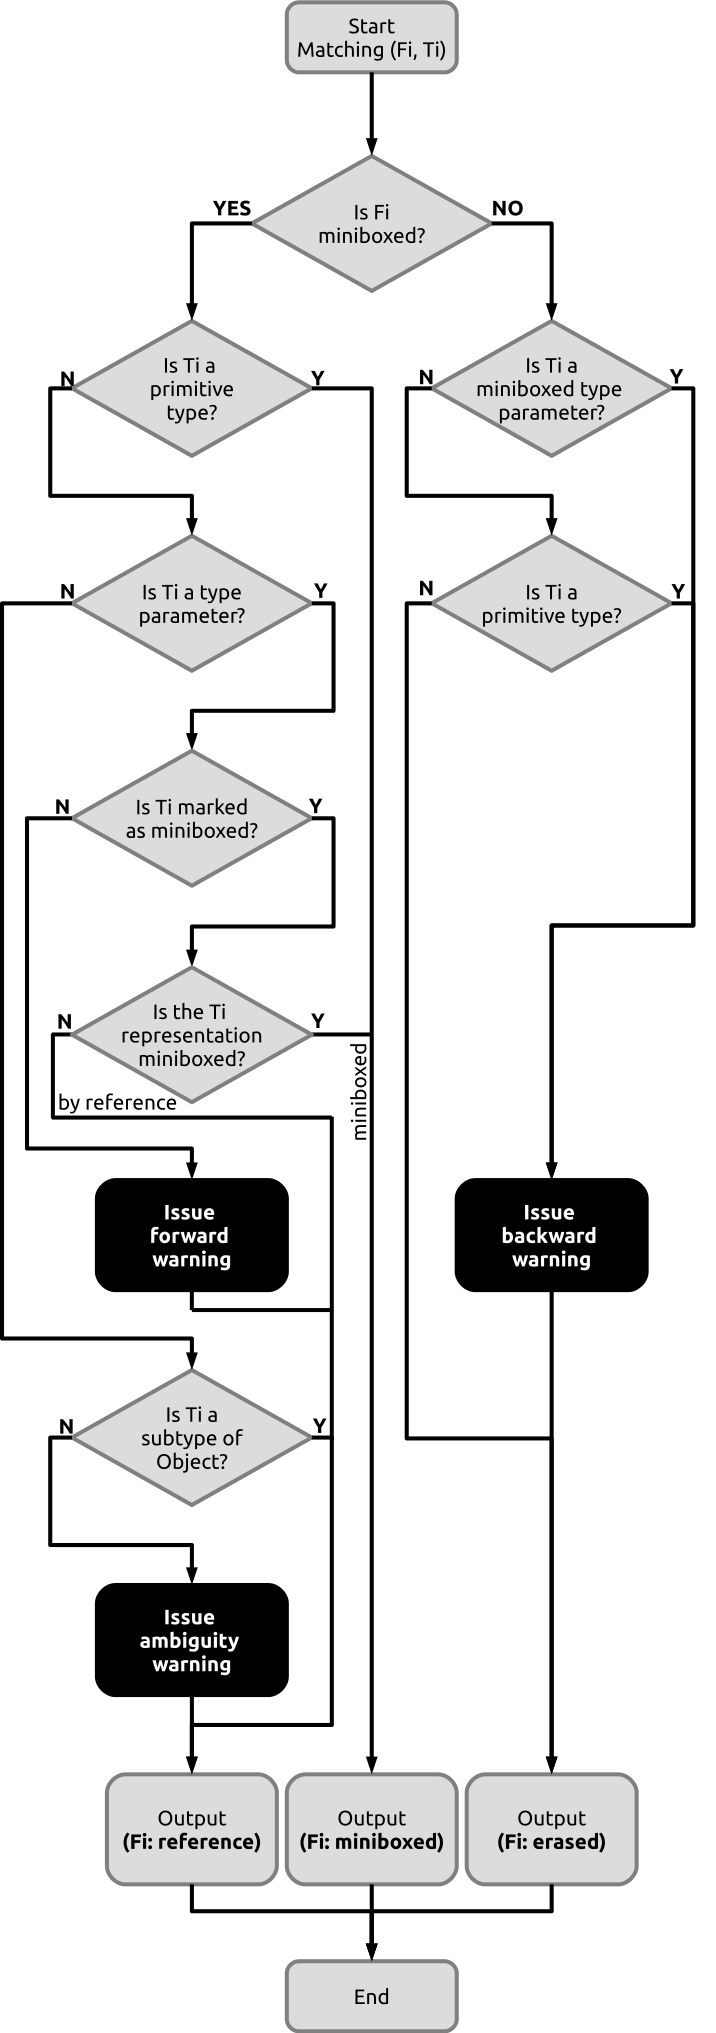
\includegraphics[height=0.91\textheight]{../graphs/warnings.pdf}
  \caption{The unification algorithm for picking the data representation of a type parameter.}
  \label{mbox2:fig:algorithm}
\end{figure}

\subsection{Unification: Formalization}

Let us call the original method or class |O|, with the type parameters |F1| to |Fn| and |VO| the set of specialized variants corresponding to |O|. Each specialized variant |V|$\in$|VO| corresponds to a mapping from the type parameters to a representation in the set of \{miniboxed, reference, erased\}. Let us inverse this mapping, to produce another mapping from type parameters and representations to the specialized variants. Let's call it |VS|.

Then the unification algorithm can be reduced to choosing the corresponding |V|$\in$|VO|, for a term of type |O[T1, .., Tn]|. This can be done following the algorithm in Figure \ref{mbox2:fig:algorithm}.

Let us take an example to illustrate this:

\begin{lstlisting-nobreak}
class C[@miniboxed M, N] // M is mboxed, N is erased
class D[L] extends C[L, Int]
\end{lstlisting-nobreak}

When deciding which specialized variant of the miniboxed class |C| to use as class |D|'s parent, we have:
\begin{itemize}
 \item the original class |O| = |C|;
 \item the type parameters |F1| = |M| and |F2| = |N|;
 \item the set of variants |VO| = \{|C_M|, |C_L|\};
 \item the inverse mapping |VS| = \{|M|: miniboxed and |N|: erased $\rightarrow$ |C_M|, |M|: reference and |N|: erased $\rightarrow$ |C_L|\}
\end{itemize}

Now, applying the unification algorithm in Figure \ref{mbox2:fig:algorithm} for the type parameter |F1| = |M| coupled with the type argument |T1| = |L|, it issues a forward warning followed by outputting (|M|: reference). Then, applying it to |F2| = |N| and |T2| = |Int|, it issues a backward warning and outputs (|N|: erased). From the two bindings, we obtain the specialized variant |C_L| to be a parent of |D|. Indeed, this is what happens in practice:

\begin{lstlisting-nobreak-nolang}
scala> class C[@miniboxed M, N]
defined class C

scala> class D[L] extends C[L, Int]
<console>:8: warning: The following code could benefit from miniboxing specialization if the type parameter L of class D would be marked as "@miniboxed L" (it would be used to instantiate miniboxed type parameter M of class C):
       class D[L] extends C[L, Int]
               ^
<console>:8: warning: The class C would benefit from miniboxing type parameter N, since it is instantiated by a primitive type:
       class D[L] extends C[L, Int]
               ^
defined class D

scala> classOf[D[_]].getSuperclass
res7: Class[_ >: D[_]] = class C_L
\end{lstlisting-nobreak-nolang}

Now it is easy to guess where the forward and backward names come from: the direction in which the miniboxing transformation propagates between the type parameter and the type argument.



\subsection{Unification: Implementation}



The performance advisories are tightly coupled with the unification algorithm, which decides the variant that should be used for transforming the code. The processing is done one step at a time, with a type parameter and type argument pair. We will now show some issues that an implementer must be careful about.



\subsubsection*{Owner chain status.} Since methods and classes in Scala can be nested in any order, we must be careful to propagate the status of the type parameters in the owner chain. In the following example:

\begin{lstlisting-nobreak}
 def a[@miniboxed A] = {
   def b[@miniboxed B] = {
     // need to be aware the representation of
     // type parameters A and B when deciding
     // which variant of C to instantiate:
     new C[A, B]()
   }
   ...
 }
\end{lstlisting-nobreak}

When deciding which miniboxed variant of class |C| to instantiate, we need to be aware of the nested methods we are located in as we duplicate and specialize the code: if we're in method |b_M| inside method |a_M|, we can rely on values of type |A| and |B| to be miniboxed. Contrarily, if we are in method |b| inside method |a|, values of type |A| and |B| are references.



\subsubsection*{Caching warnings.} Instead of issuing warnings right away, they are being cached and later de-duplicated. The reason is that issuing too many warnings diminishes their value. Aside from the three advisories shown, there are special advisories dealing with the specialization transformation in Scala and certain library constructs that we show in the next section. Thus, we define an ordering of advisory priority and, if multiple warnings are cached, we only issue the most important ones.

\subsubsection*{Suppressing warnings.} In certain scenarios, programmers are aware of their sub-optimal erased generic code but, due to compatibility requirements with other JVM programs or due to the fact that code lies outside the hot path, they chose not to change it. In these situations, they need to suppress the warnings, because instead of improving visibility, they might obscure other more important performance regressions in the program. However, a coarse-grained approach such as turning off all warnings is not desirable either, as it completely voids the benefit of advisories. For this scenario, the miniboxing transformation provides the |@generic| annotation, which can suppress performance advisories:

\begin{lstlisting-nobreak}
 scala> def zoo[`@miniboxed` T](t: T) = t
 defined method zoo

 scala> zoo[Any `@generic`](3) // no ambiguity warning
 res1: Any = 3

 scala> def boo[`@generic` T](t: T) = t
 defined method boo

 scala> boo[Int](3)                   // no backward warning
 res2: Int = 3
\end{lstlisting-nobreak}



\subsubsection*{Libraries.} In other cases boxing is caused by the interaction with erased generics from libraries. In this case, the default decision is not to warn, unless the programmer specifically sets the |-P:minibox:warn-all| compiler flag:

\begin{lstlisting-nobreak-nolang}
 scala> 3 :: Nil
 <console>:8: warning: The method List.:: (located in scala-library.jar) would benefit from miniboxing type parameter B, since it is instantiated by a primitive type:
               3 :: Nil
                 ^
 res0: List[Int] = List(3)
\end{lstlisting-nobreak-nolang}

As we will see in the benchmarking section (\S\ref{mbox2:sec:bench}), the performance advisories allow programmers who are not familiar with the transformation to make the same changes an expert would do.
